\chapter{SIMULACIONES CON DISTINTOS COEFICIENTES DE DILATACIÓN ADIABÁTICA}
\label{cap:5}
En este último capítulo se comparan los resultados obtenidos en simulaciones del mismo problema de condición inicial pero con distinto coeficiente de dilatación adiabática $\gamma$, con el fin de obtener una intuición física, a través de la simulación, de cómo varía el comportamiento de un gas cuando el número de grados de libertad interno del mismo cambia.
\section{Consideraciones preliminares}
Dado que el coeficiente de dilatación adiabática está relacionado explícitamente con el número de grados de libertad interno de un gas ($\alpha$),
\begin{equation}
	\gamma = \frac{\alpha + 2}{\alpha},
\end{equation}
es conveniente definir los valores para $\gamma$ tal que dependan de un valor entero para $\alpha$.

En las anteriores simulaciones, se calculó $\gamma$ para un gas diatómico, como el aire. La justificación del número de grados de libertad de estos gases se dio en la sección \ref{sec:ecuacion-de-estado-gas}. En este caso:
\begin{equation}
	\alpha = 5 \implies \gamma = 7/5 = 1.4.
\end{equation}
Si se considera un gas monoatómico, entonces éste contaría con tres grados internos de libertad traslacional únicamente, obteniendo $\gamma=5/3$. 

Por otro lado, modelando un gas cuyas moléculas constituyentes poseen 4 grados de libertad rotacionales, 3 traslacionales y 2 vibracionales, se tendría $\alpha=9$, mientras que $\gamma=11/9$.

Entonces, se considerarán experimentos con gases de 3, 5 y 9 grados de libertad
internos, que corresponden a $\gamma = 5/3$, $\gamma = 7/5$ y $\gamma = 11/9$ respectivamente.
%Entonces, se considerarán experimentos con gases de 16 y 32 grados de libertad internos, que corresponden a $\gamma=1.125$ y $\gamma=1.0625$ respectivamente.
\section{Test de Sod}
El problema de condiciones iniciales que se estudiará con simulaciones con distintos valores para $\gamma$ es el test de Sod (sección \ref{sec:sod_con_entropy148}). En las figuras \ref{fig:sod-gammas-1} - \ref{fig:sod-gammas-2} se encuentran seis instantes temporales de las simulaciones para el test de Sod.
\begin{figure}[H]
	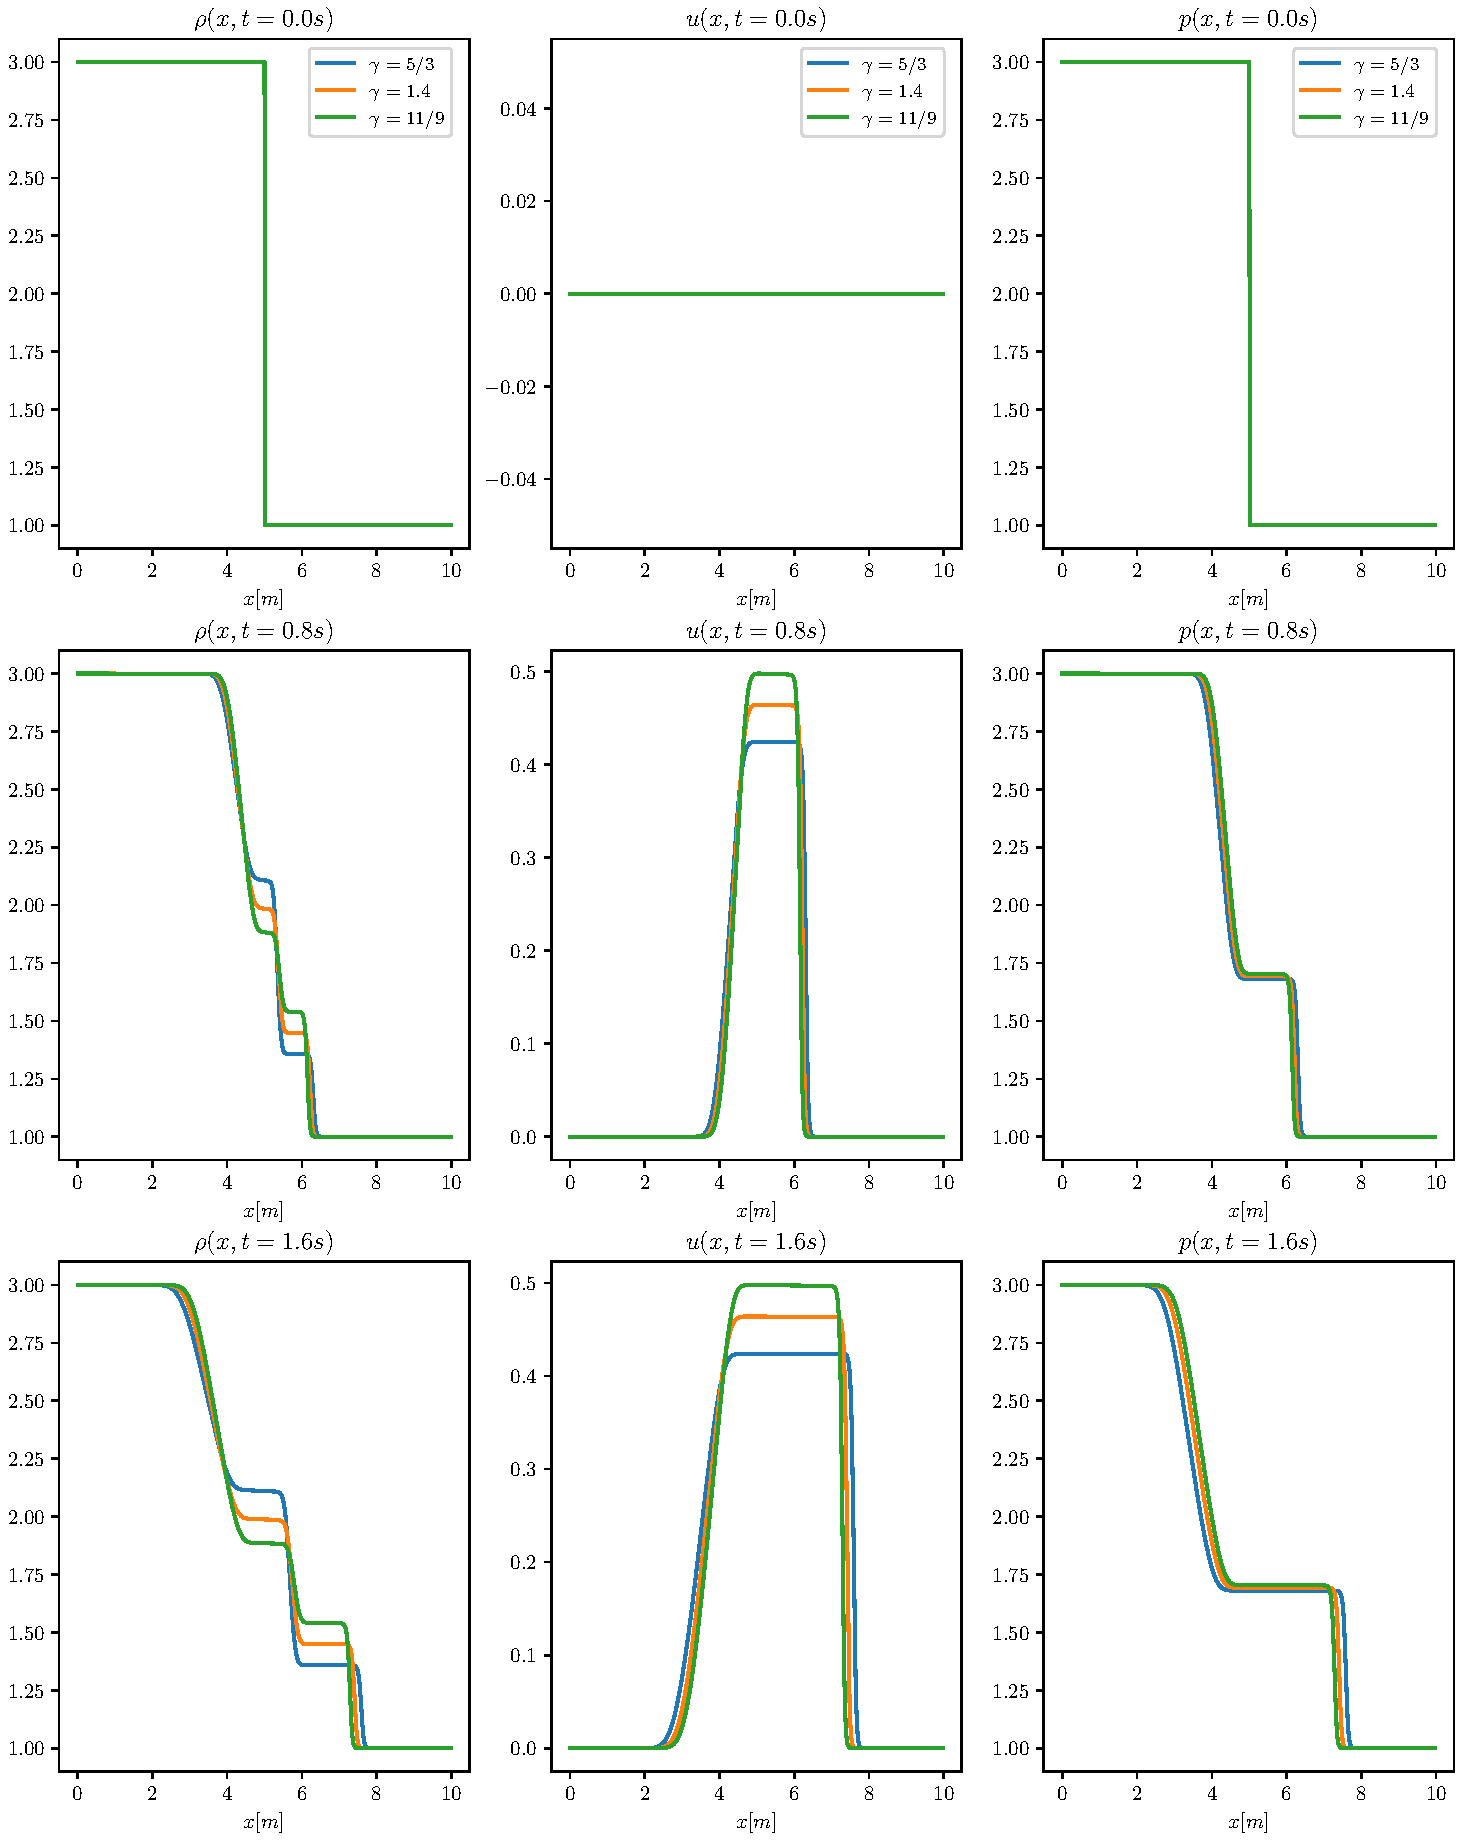
\includegraphics[width=0.95\linewidth]{../euler1D/experimentos/graficas_sod/1.pdf}
	\caption{Primeros tres instantes de las simulaciones con distintos $\gamma$.}
	\label{fig:sod-gammas-1}
\end{figure}
\begin{figure}[H]
	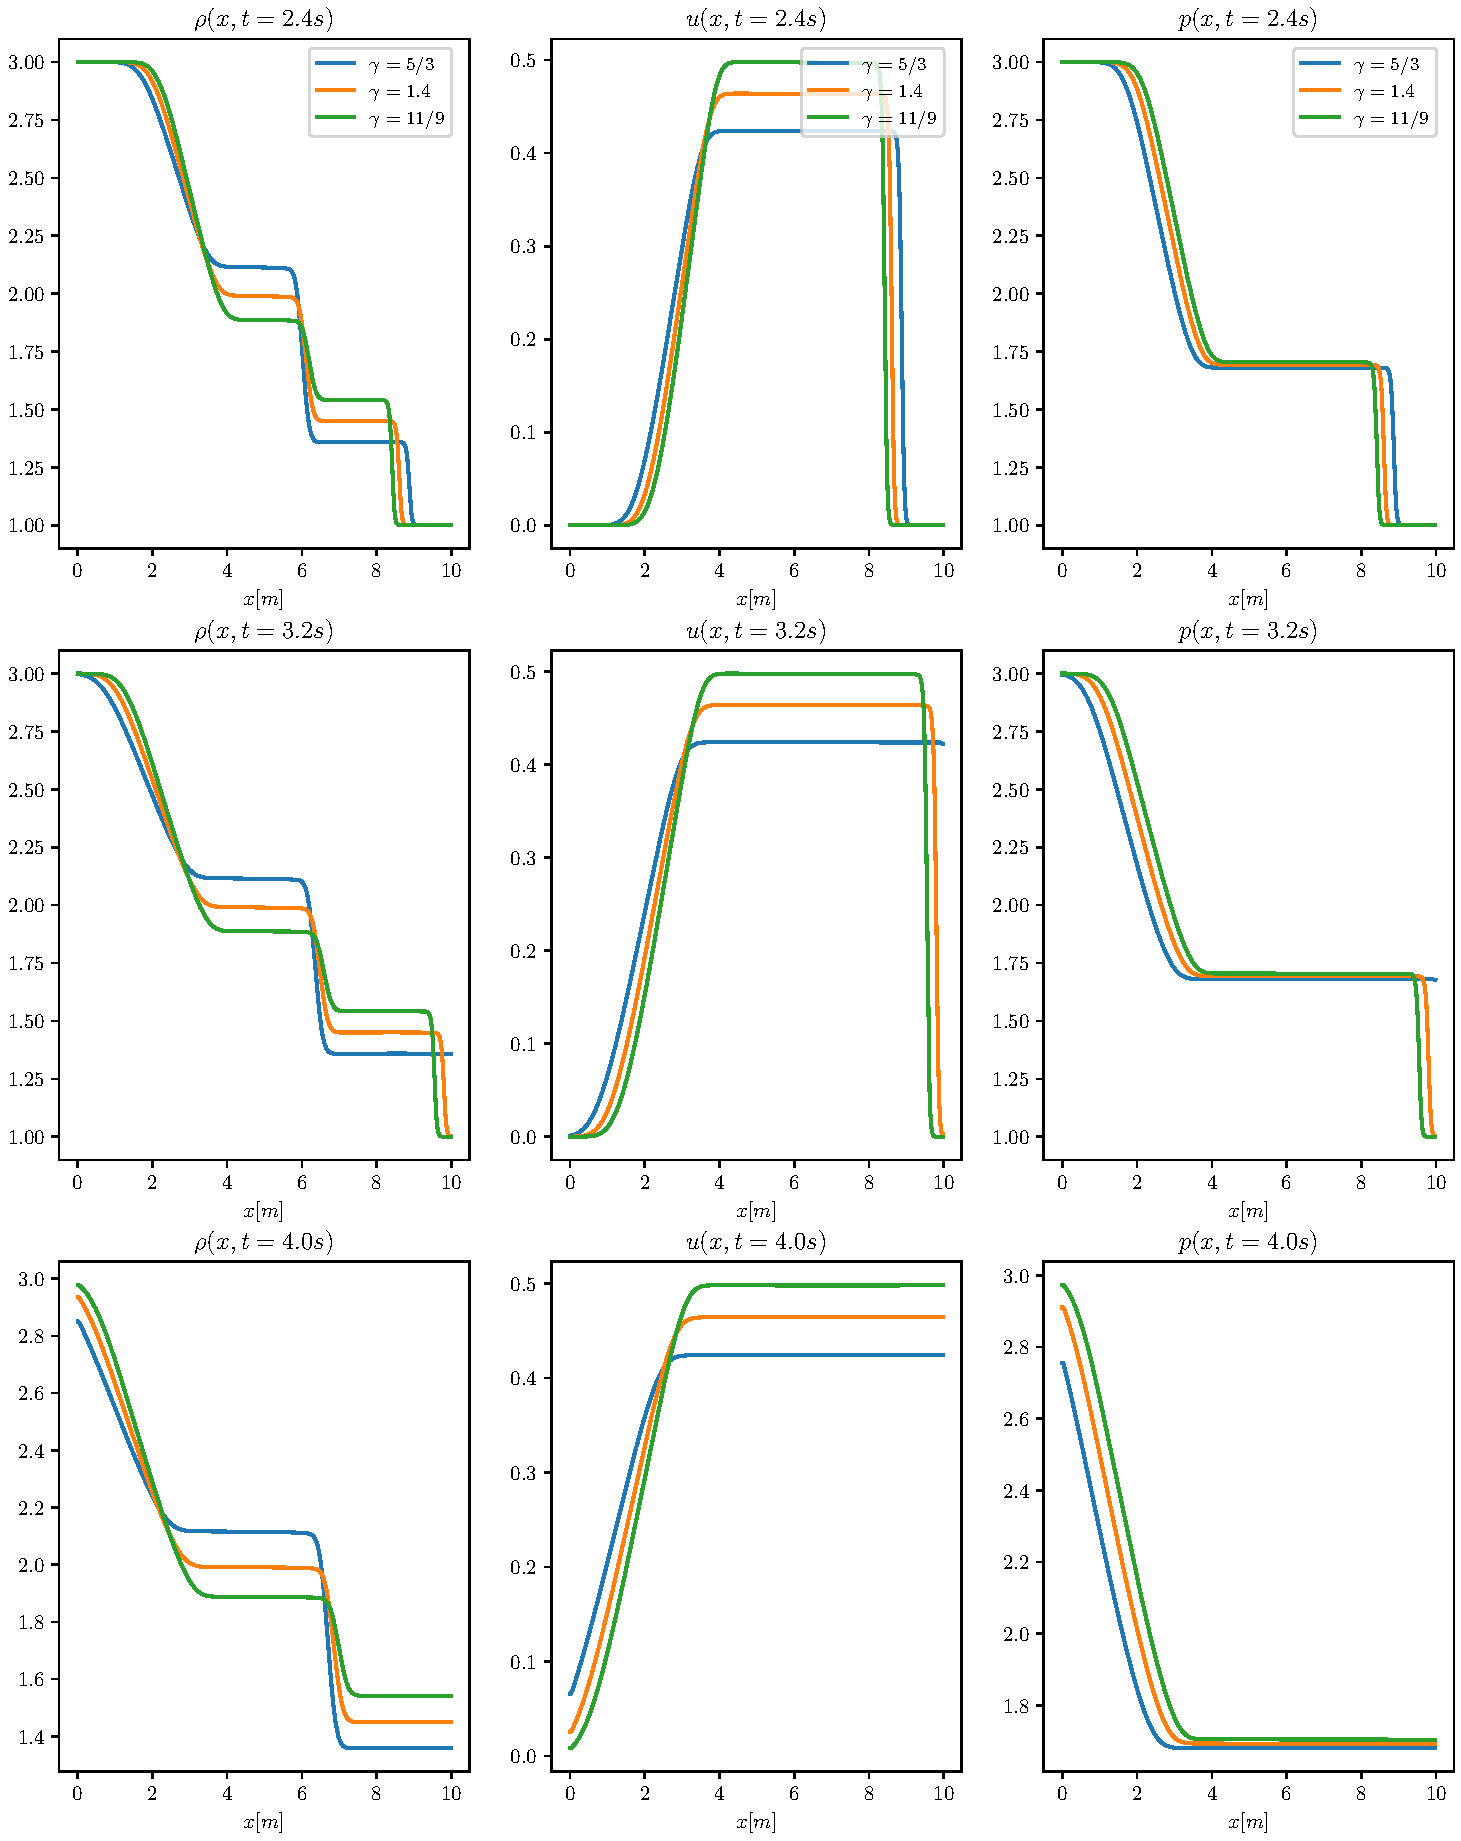
\includegraphics[width=\linewidth]{../euler1D/experimentos/graficas_sod/2.pdf}
	\caption{Últimos tres instantes de las simulaciones con distintos $\gamma$.}
	\label{fig:sod-gammas-2}
\end{figure}

\subsection{Observaciones}
\begin{itemize}
	\item En la simulación para la densidad, destaca cómo la diferencia en la discontinuidad de contacto disminuye al disminuir $\gamma$. Se puede hipotetizar que en el límite $\alpha \rightarrow \infty$, la discontinuidad de contacto desaparece completamente. De acuerdo a \cite{LeVeque}, cuando $\gamma = 1$, la simulación correspondería a la de un gas con \textbf{flujo isotérmico}. Esto último es consistente con la desaparición de la discontinuidad de contacto, ya que esta aparece cuando dos partes del gas tienen temperaturas distintas.
	\item Se destaca que las velocidades de los gases alcanzan distintos valores máximos; mientras más cercano a 1 es el valor de $\gamma$ mayor es el valor de la velocidad $u$. Sin embargo, la velocidad de propagación de esta discontinuidad es distinta para cada gas y sucede al contrario que con la última observación. A mayor $\gamma$, mayor velocidad de propagación.
	\item La presión destaca por ser la cantidad que menos varía entre los gases simulados. La principal diferencia entre las presiones es, al igual que con la velocidad, la velocidad de propagación de las ondas. Esto sucede tanto con la onda de choque como con la de rarefacción.
\end{itemize}

\subsection{Entropía y energía}
La entropía de un gas regido por las ecuaciones de Euler, está definida por
\begin{equation}
	S = c_{v}\log(p/\rho^{\gamma}) + \text{constante},
\end{equation}
donde $c_v$ es la capacidad calorífica específica a volumen constante \cite{LeVeque}. En las figuras \ref{fig:ee-gammas-1} - \ref{fig:ee-gammas-2} se muestran las gráficas correspondientes a la energía total \eqref{eq:energia-total} y la entropía, para cada gas, en seis instantes de tiempo. La entropía se calculó y graficó en unidades de $c_v$ y con la constante arbitraria igual a 0.


\begin{figure}[H]
	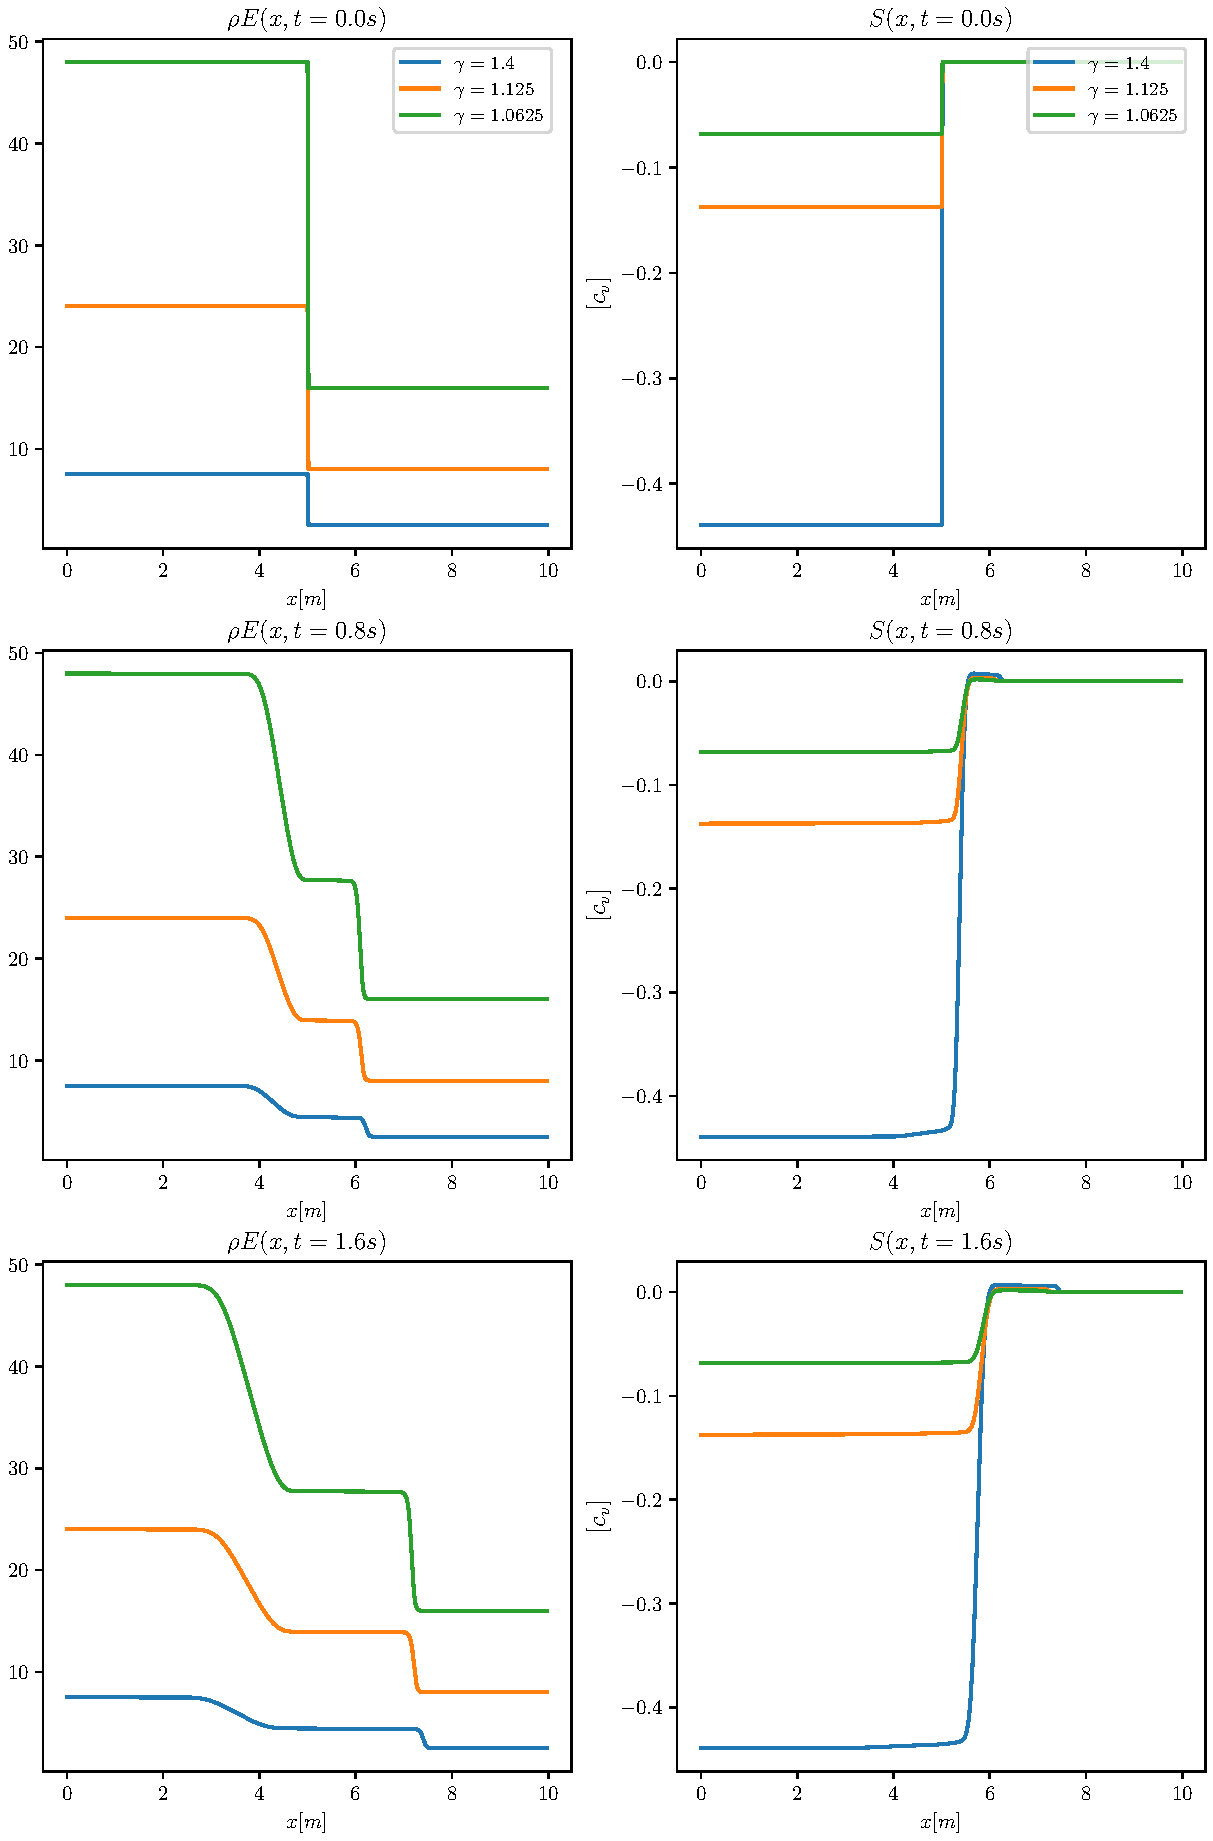
\includegraphics[width=\linewidth]{../euler1D/experimentos/energia/1.pdf}
	\caption{Energía y entropía en los primeros tres instantes de las simulaciones con distintos $\gamma$.}
	\label{fig:ee-gammas-1}
\end{figure}
\begin{figure}[H]
	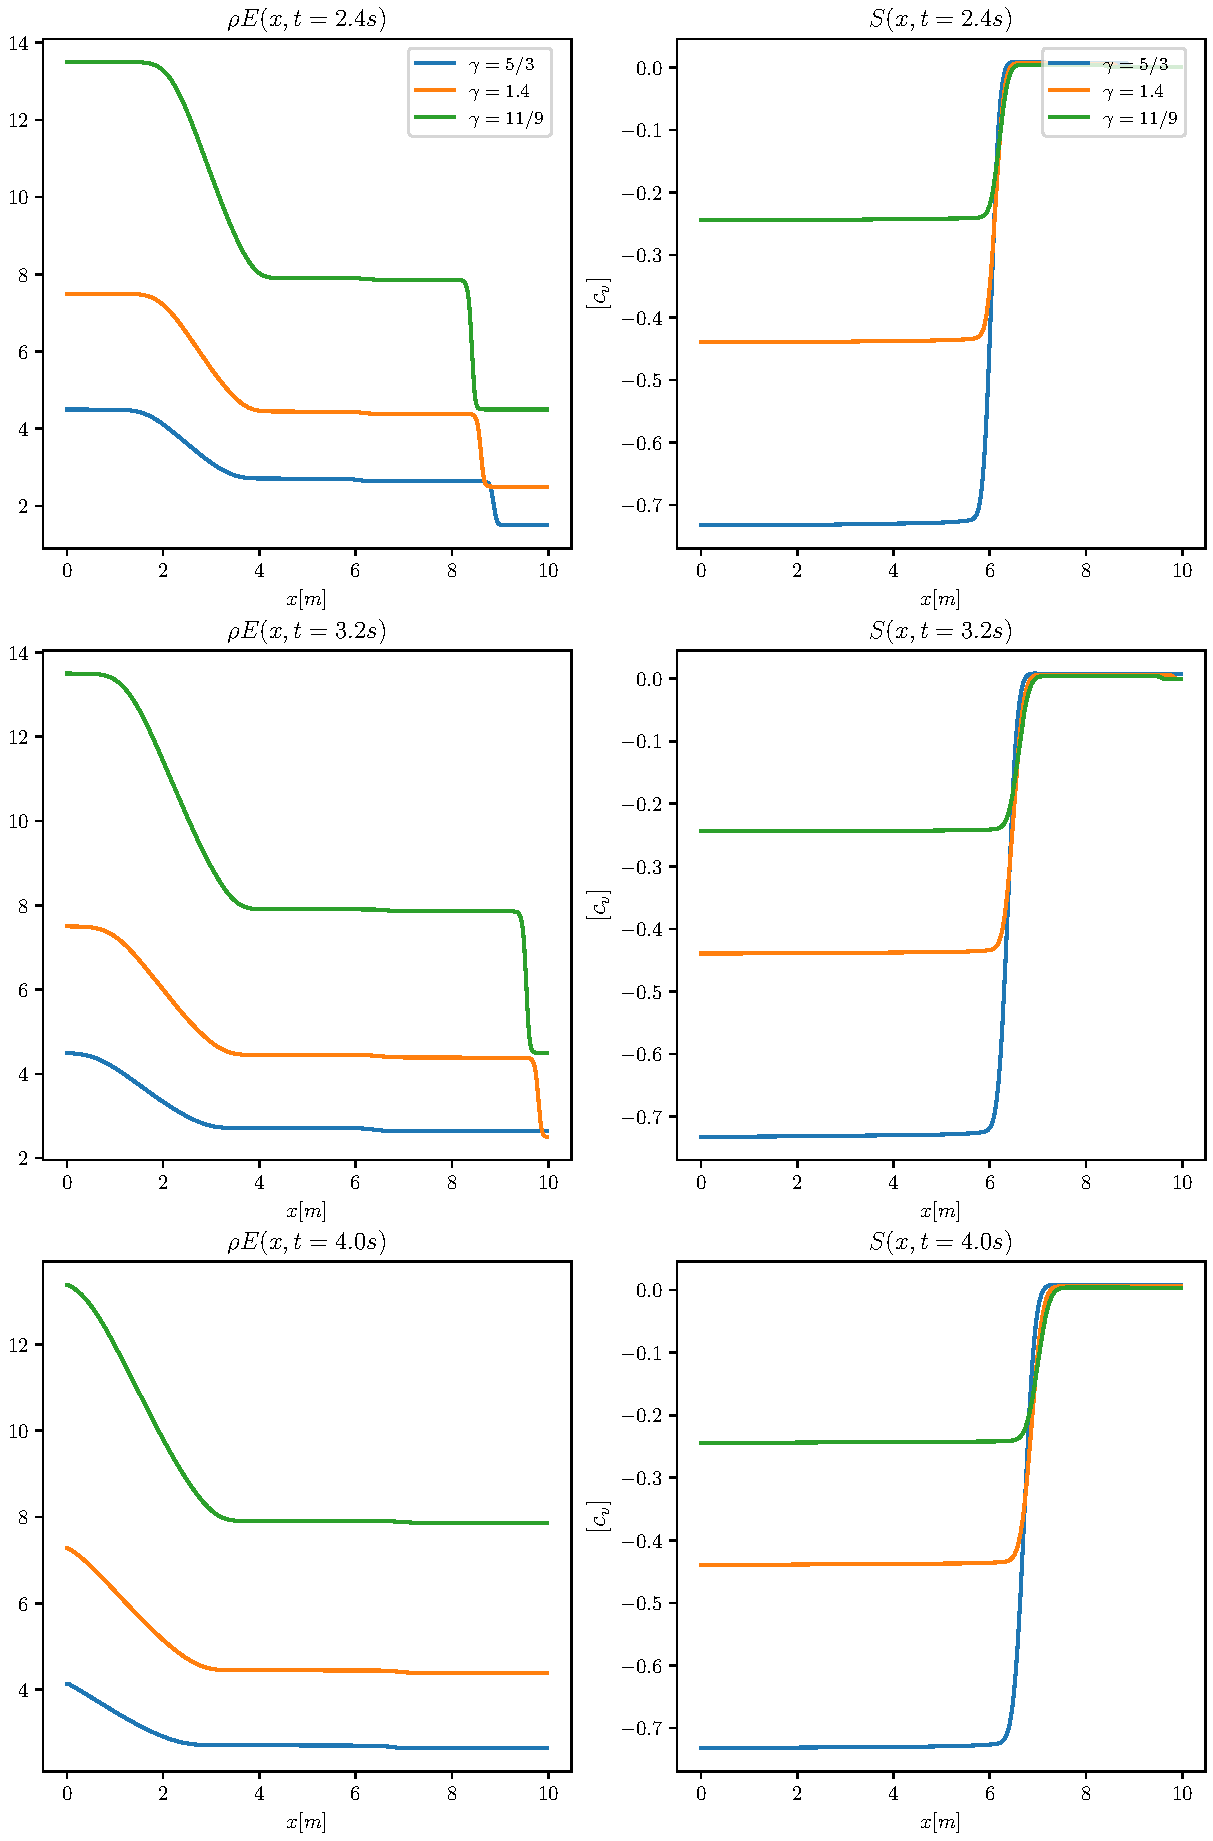
\includegraphics[width=\linewidth]{../euler1D/experimentos/energia/2.pdf}
	\caption{Energía y entropía en los últimos tres instantes de las simulaciones con distintos $\gamma$.}
	\label{fig:ee-gammas-2}
\end{figure}

Se pueden destacar las siguientes observaciones encontradas a través de las gráficas de energía y entropía:
\begin{itemize}
	\item La energía presenta la mayor diferencia entre los gases simulados, lo cual era esperado ya que la energía total depende explícitamente de $\gamma$. La gráfica de la energía se parece a la de presión, en el sentido que presenta una onda de rarefacción, que se traslada hacia la izquierda, y una onda de choque que se traslada hacia la derecha. Esta última característica también era esperada dado que la energía interna depende linealmente de la presión. La energía cinética contribuye principalmente a la onda de choque presentada en la energía total.
	\item La solución producida para la entropía destaca por coincidir con una onda de choque. La entropía tiene a ser constante mientras avanza la evolución temporal. La diferencia entre la entropía de cada gas es considerable dado que ésta también depende de $\gamma$.
	\item Otro hecho demostrado con la simulación es que la entropía de un gas con mayor $\alpha$ (menor $\gamma$) siempre es mayor que la entropía de un gas con  menor $\alpha$. Es sencillo justificar esta observación, puesto que cuando existen más grados de libertad internos disponibles, la energía puede repartirse de más formas; logrando así un incremento en la entropía. 
\end{itemize}